\chapter{Estimation Theory}
\section{Introduction to Data Analysis}
\subsection{Data Analysis}
Data Analysis is the process of extracting information from data. Although data and information are often used interchangeably, they are not the same. Data is something that should cointain information, but it is not information itself. In order to extract information from data, we need to build a learning system.

An important thing to know is that when the learning system is \textit{good}, then by increasing the amount of data we have, the available information cannot decrease. In practice, most of the times we do not have a good system (due to analytical, computational, or time skills not available), so it can happen that the data fed to the system is misleading and the information we get from the analysis decreases. A \textit{non optimal} system could be attacked using fake data in order to decrase information and make the system less reliable; the \textit{optimal} system is able to discard that data.

The two main families of problems in data analysis are \textit{estimation} and \textit{classification}. The main difference is that in the estimation problem,
we have a set of data and we want to estimate a real value, while in the classification problem the output is contained in a finite set. This difference is projected onto the output response variable $Y$.

\begin{figure}
    \centering
    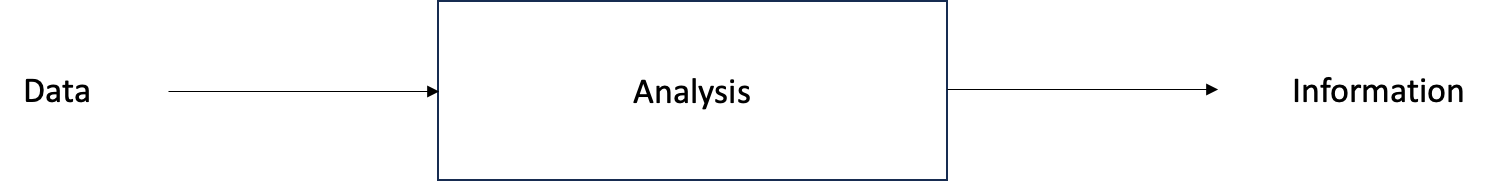
\includegraphics[width=0.7\textwidth]{./figures/chapter_2/data2information.png}
    \caption{The general process of extracting information from data.}
    \label{fig:data2information}
\end{figure}

The input of the learning system can be anything (a vector, a matrix, a graph, a sequence, etc.), but the output is always a real number or a finite set of values. In general,
we do not care about the dimension of the output, because we can always repeat the problem as many times as the dimension of the output.

% qualcosa sul fatto che esiste model based analysis e supervised parametric e non parametric

Data analysis problems don't necessary require a \textit{training phase}. We can have two scenarios:
\begin{enumerate}
    \item \textbf{Model-Based}, the model is given to us.

        \begin{figure}
            \centering
            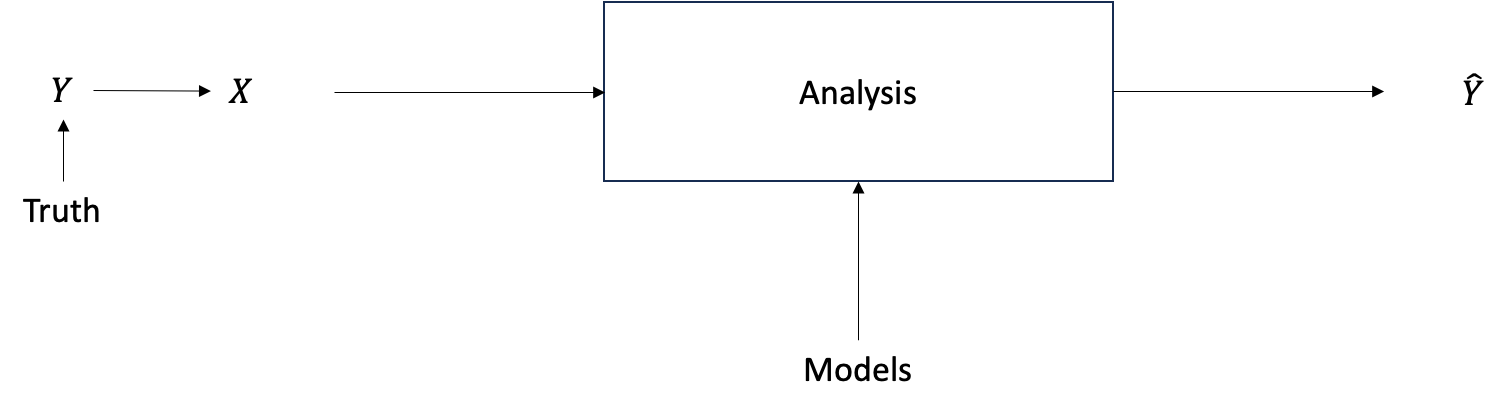
\includegraphics[width=0.7\textwidth]{./figures/chapter_2/modelbased.png}
            \caption{The model based process of extracting information from data.}
            \label{fig:modelbased}
        \end{figure}

        Figure \ref{fig:modelbased} show the scenario. The truth $Y$ influences the data $X$, hidden in it.

        \callout{Note}{Another thing to make clear is that in statistical learning, we do not have a temporal correlation between the variables. When we say that two variables depend on each other, we just mean that they are correlated, without implying the causality.}

    \item \textbf{Model Learning}, we have to learn a statistical characterization of the couple $(X,Y)$. 
        
        \begin{figure}
            \centering
            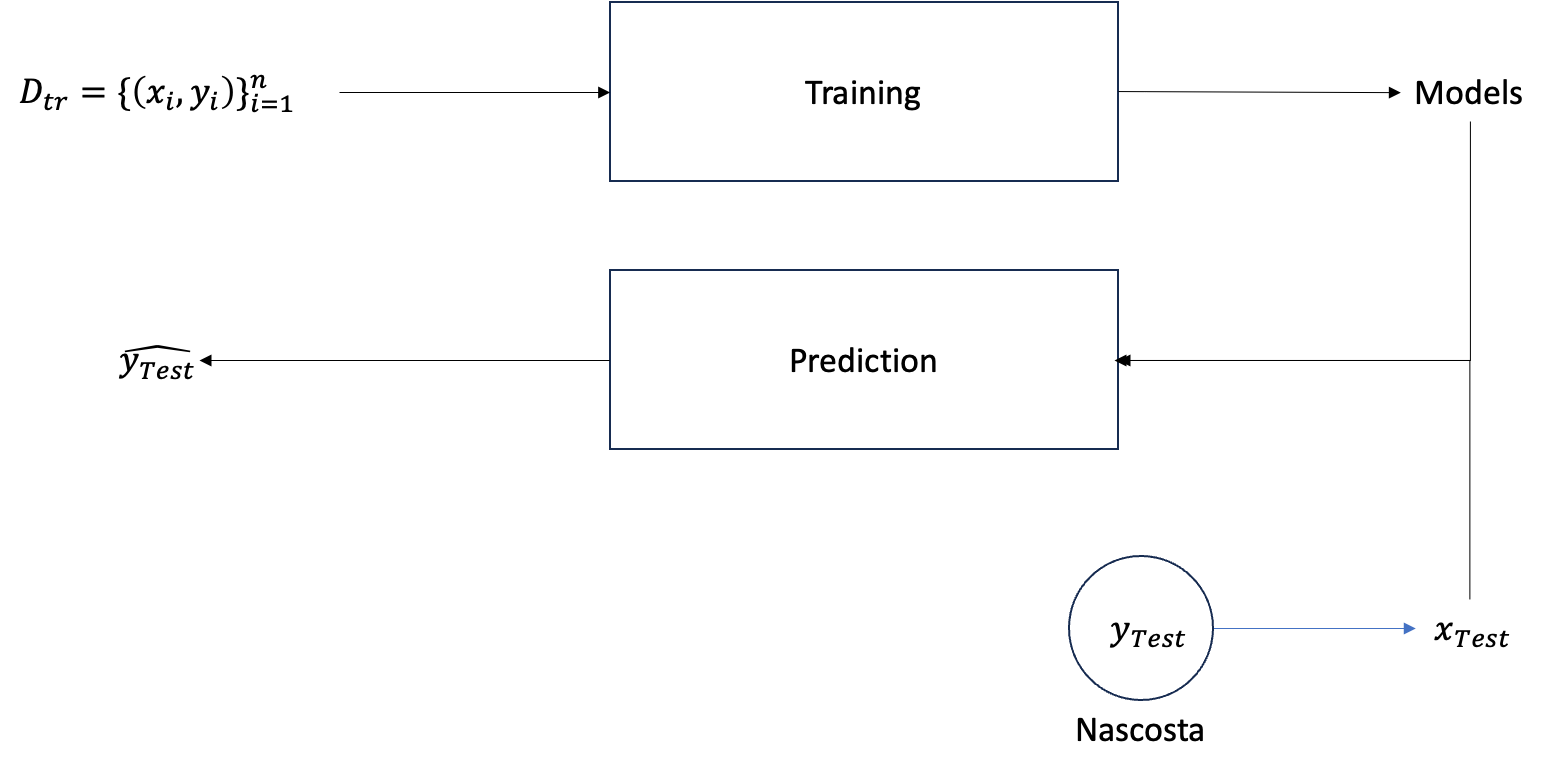
\includegraphics[width=0.7\textwidth]{./figures/chapter_2/modellearning.png}
            \caption{The model learning process of extracting information from data.}
            \label{fig:modellearning}
        \end{figure}

        This scenario could be seen as a \textit{supervised learning} problem when we starts from a set of examples $\mathcal{D}$ to learn the model.
        \[
            \mathcal{D} = \left\{ x_i, y_i \right\}_{i=1}^{N}
        \]
        Figure \ref{fig:modellearning} explain this scenario. 


\end{enumerate}

\section{Bayes Estimation}
\subsection{Random variable approximation}
Assume we have a random variable $Y$ and we want to approximate it with a single deterministic value. To do that, we need to find the number that, on average, is the closest to the values of the random variable. In other words, we want to find the number $z^\ast$ that minimizes the expected value of the \textit{distance} between $Y$ and $z$:
\[
    z^\ast \colon \arg \min_{z \in \mathbb{R}} \E{}{(Y-z)^2}
\]
\callout{Why the squared difference?}{There are multiple reasons. The first one is that in this way the error is always positive and has a unique minimum in 0. The second reason is that the square term is the first even power and is differentiable everywhere.}
The quantity we want to minimize is called \textit{mean squared error} (MSE) and in this case is a function of the value $z$. 
We can find the minimum of this function by computing its derivative and setting it to zero:
\[
    f(z) = \E{}{(Y-z)^2}
\]
By leveraging the linearity of the expectation, we can write:
\[
    f^{\prime} (z) = 0 \Leftrightarrow \E{}{\frac{d}{dz} (Y-z)^2} =  \E{}{-2(Y-z)} = -2\E{}{Y} - 2z = 0 \iff z^{\ast}  = \E{}{Y}
\]
Another typical approach to solve the problem without using the derivative is by introducing $\mu$ inside the function:
\begin{align*}
    f(z) &= \E{}{(Y-z)^2} = \E{}{(Y - \mu + \mu - z)^2} = \\
    &= \E{}{(Y - \mu)^2} + 2\E{}{(Y - \mu)(z - \mu)} + (z - \mu)^2 = \\
    &= \var{Y} + (z - \mu)^2
\end{align*}
% \[
%     f(z) = \E{}{(Y-z)^2} = \E{}{(Y - \mu + \mu - z)^2} = 
% \]
% \[
%     = \E{}{(Y - \mu)^2} + 2\E{}{(Y - \mu)(z - \mu)} + (z - \mu)^2
%     = \var{Y} + (z - \mu)^2
% \]
The obtained function is composed by a $z$-dependent term that is the \textbf{reducible} part and a constant term as \textbf{irreducible} part. This is a very common pattern. 
So, the minimum of the function is equal to $\var{Y}$ and is reached when the second term is zero, that is, as we expect:
\[
    z^{\ast} = \mu
\]

\subsection{MMSE}
Suppose we want to estimate the response $Y$ using the data $X\in\R^d$.
For that purpose we want to find a function of the data $g(X)$ that is the best approximation of $Y$ as represented in figure \ref{fig:mmseestimation}.

\begin{figure}
    \centering
    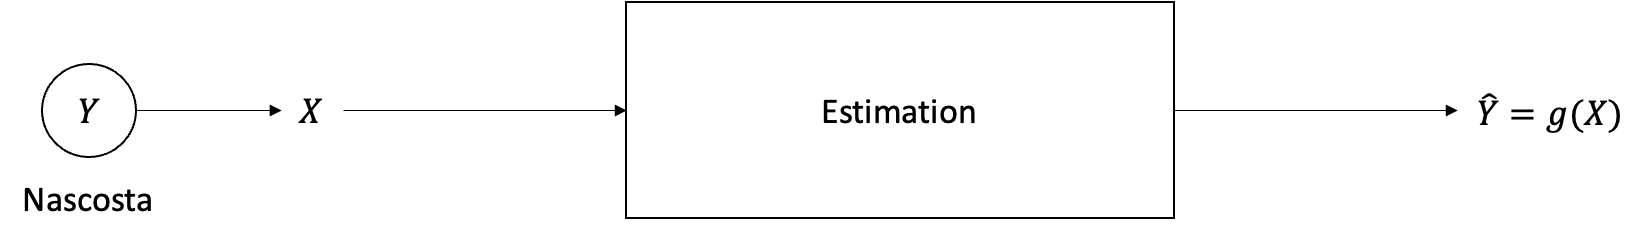
\includegraphics[width=0.7\textwidth]{./figures/chapter_2/mmse.png}
    \caption{The estimation process using $g(X)$.}
    \label{fig:mmseestimation}
\end{figure}

We can still minimize the MSE to obtain the optimal function $g^\ast(X)$:
\[
    g^\ast(X) = \arg\min_{g \in\mathcal{G}} \E{}{(Y-g(X))^2}
\]
The MSE function is a function of both $Y$ and $X$, so the expectation is not well defined. To solve this problem, we would need to first solve fixing $X$, so that $g(X)$ is constant, then linking the conditioned result to the original problem. This can be done by applying the \textbf{tower property}:
\[
    g^\ast(X) = \arg\min_{g \in\mathcal{G}} \E{X}{\E{Y}{(Y-g(X))^2 \mid X}}
\]

The inner expectation is a function of $Y$ only since $g(X)$ is now constant. By minimizing the inner expectation we find the value of the function $g$ assumed for a specific value of $X$. By doing it for each value of $X$ we could construct $g(X)$.
In reality, if we do minimization for each value of $X$, we are doing something stronger than the minimization of the MSE, because we are minimizing the MSE for each value of $X$.
For this reason, we can also avoid to compute the outer expectation and we can write:
% The inner expectation is a function of $Y$ only, so we can apply the same reasoning as before and find that the function that minimizes the inner expectation is the mean of $Y$: $\E{Y}{Y}$. So we have:
\[
    g^\ast(X) = \E{Y}{Y \mid X = x} \triangleq \hat{Y}_{MMSE}
\]
which is the conditional mean of $Y$ given $X$ and it is also called \textbf{posterior mean} because it is the mean of the posterior distribution $f(y|x)$.
Since it is the minimum of the MSE, it is also called \textbf{minimum mean squared error} (MMSE) estimator.

\section{Maximum Likelihood Estimation}
In the bayesian setting the parameter was a random variable. Now let us consider the case in which the parameter is a deterministic quantity, but it is unknown.

Assume that we have a random variable $X \in \mathbb{R}^d$ that is generated by an unknown distribution that depends on a parameter $\theta \in \mathbb{R}$.

The parameter can be considered as the \textit{truth} that generates the data and we want to find an estimator $\hat{\theta}$ for $\theta$ that is a function of the data $X$.

\begin{figure}
    \centering
    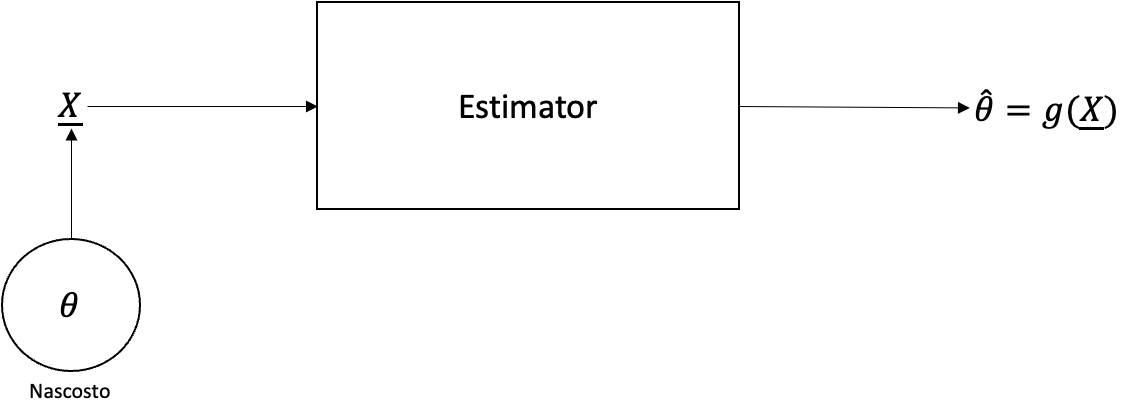
\includegraphics[width=0.7\textwidth]{./figures/chapter_2/mlprocess.png}
    \caption{The estimation process of a deterministic parameter.}
    \label{fig:mleestimation}
\end{figure}

As \textbf{error metric} we can use, again, the \textit{mean squared error}:
\[
    h(\theta) = \E{}{(\theta - \hat{\theta})^2} = \E{}{(\theta - g(X))^2} = \sum_{x \in X} p(x) (\theta - g(x))^2
\]
In the bayesian setting the error metric was the following:
\[
    h(Y,X) = \E{}{(Y-g(X))^2}
\]
The difference between the two error metrics is that in the first case, the expression is a function of $\theta$, in the second case the expression is a number, because the expectation of a random variable is a scalar value by definition.

If we want to minimize the error metric $h(\theta)$, we could compute a degenerate solution that is $g(X) = \theta$. In this case the error will be zero, but we would reach a contradiction, because that would mean that we already know $\theta$, which is not true because it is our parameter.

In order to find out an estimator, we apply the \textbf{maximum likelihood} strategy.  
Since the previous way can't be afforded, we need to use different paradigms and assumptions.
The maximum likelihood strategy starts from the assumption that the estimator $g(X)$ is \textbf{unbiased} (condition of \textit{unbiasedness}).
Thinking about, it's reasonable to assume that the expected value of the estimator of the parameter is equal to the parameter itself.
\begin{definition}
    The likelihood function $\ell(x;\theta)$ is the joint probability mass or density function of the data and the parameters of the model.

    When we consider a realization of the random variable $X$ that represents the data, the likelihood function is a function of the parameter $\theta$:
    \[
        \ell(x | \theta) = \mathbb{P}(X = x | \theta)
    \]
    which can be seen as the probability mass or density function of the data $X$ given the parameter $\theta$.
\end{definition}

\begin{theorem}
    In order to find the \textbf{maximum likelihood estimator}, we need to find the value of $\theta$ that maximizes the likelihood function.
    \[
        \hat{\theta}_{ML} = \arg\max_{\theta} \ell(x; \theta)
    \]
\end{theorem}

Assume that we know the shape of the likelihood functon. In order to find a point of maximum we need to solve the following equations:
\begin{align*}
    \frac{\partial \ell(x;\theta)}{\partial \theta} = 0 \\
    \frac{\partial^2 \ell(x;\theta)}{\partial \theta^2} \geq 0
\end{align*}
The equations have a closed form solution only if the likelihood function is derivable. If the likelihood function is not derivable, we need to use a gradient ascent algorithm. However, the latter is not garanteed to always work, because in order for the solution of the algorithm to converge to the point of true maximum we need jumps that are proportional to the derivative, decreasing the learning rate.

Another simple strategy is to use a brute-force algorithm that tries all the possible values of $\theta$ and finds the one that maximizes the likelihood function. This is a bit more complex in continuous case since we have to discretize the space of $\theta$.

In any case, it depends on the \textit{shape} of the likelihood function; for example there may be a \textit{subgradiant shape} or there may be a situation in which we have local maxima and minima.

\paragraph*{High dimensional parameters}
The \textit{maximum likelihood strategy} works also if the parameter is a vector. If $\vec{\theta} \in \mathbb{R}^m$ we will find that:
\[
    \hat{\vec{\theta}} = \arg\max_{\vec{\theta}}  \ell(x; \vec{\theta})
\]
However, we should be careful while increasing the dimension of the parameter, because of \textit{curse of dimensionality problem}; we have an exponential dependence between the number of dimensions and the number of elements in the dataset.

\paragraph*{Properties of the Maximum Likelihood Estimator}
Maximum likelihood estimators are also called Minimum-Variance Unbiased (\textit{MVU}) estimators. This is because, given independent data, they are:
\begin{enumerate}
    \item asymptotically unbiased
    \item asymptotically efficient, meaning that they find the estimate with minimum variance. The minimum value of variance is bounded by the \textbf{Cramer-Rao lower bound}, that is defined by the Fischer Information matrix.
    \item have \textbf{large-sample optimality}, meaning that it is optimal if we have many data, independently of the particular problem.
\end{enumerate}

\callout{Note}{The maximimum likelihood estimator has a lot of nice \underline{asymptotic} properties, namely it works well with a high availability of data. By the way, it make also sense to use it with a small amount of data, because it is a reasonable estimator with theoretical foundamentals and we can't do better.}

\section{Exercises}
\subsection{Maximum Likelihood}
\subsection{Mean estimation on homogeneous data}
\begin{exercise}
    Compute the maximum likelihood estimator for the mean of a gaussian random variable with known variance.
\end{exercise}
Given data $X \in \mathbb{R}$ and variance $\sigma^2$, the likelihood function is:
\[
    \ell(x;\theta) = \frac{1}{\sqrt{2\pi\sigma^2}} \exp{-\frac{(x-\theta)^2}{\sigma^2}}
\]
In this special case, the likelihood function for a fixed $X$ has the same shape of the probability function of $X$, $f(x)$. 
It is intuitive, by looking at the curve that the point of maximum is the mean of the distribution, that is the parameter $\mu$.

Applying the strategy at the monodimensional case, we have:
\[
    \hat{\theta}_{\text{ML}} = \arg\max_{\theta} \ell(x; \theta) = x
\]
Intuitively, if we have a single data point, the best estimate for the mean is the data point itself.

Let us now consider the case when $X$ becomes a vector. We have that $X \in \mathbb{R}^N$, where
$X = \left[x_1, \dots, x_N\right]^T$ are all \textit{iid} guassian random variables and $\sigma^2$ is known. We need to compute the joint PDF of all of the variables. In the case of independent variables, the joint PDF is the product of the PDFs of each variable:
\begin{align*}
    \ell(\vec{x};\theta) = \prod_{i=1}^{N} \ell(x_i;\theta) = \prod_{i=1}^{N} \left(\frac{1}{\sqrt{2\pi\sigma^2}} \exp{-\frac{(x_i - \theta)^2}{2\sigma^2}}\right) \\
    = \left(\frac{1}{\sqrt{2\pi\sigma^2}}\right)^n \exp{-\frac{\sum_{i=1}^{N} (x_i - \theta)^2}{2\sigma^2}}
\end{align*}
The constant is irrelevant to find the point of maximum; so we have:
\[
    \exp{-\frac{\sum_{i=1}^{N} (x_i - \theta)^2}{2\sigma^2}}
\]
But the maximum value of the exponential function is found for the minimum value of its exponent, because this function is monotonically decreasing. So, ignoring the constants, we have that the argmax of the likelihood function in this case is equivalent of the argmin of its exponent:
\[
    \arg\max_{\theta} - \sum_{i = 1}^{n} {(x_i - \theta)^2} \Leftrightarrow \arg\min_{\theta} \sum_{i = 1}^{n} {(x_i - \theta)^2}
\]
Now we need to compute the derivative wrt $\theta$ and equate to zero:
\begin{gather*}
    \frac{\partial }{\partial \theta}\sum(x_i-\theta)^2 = 0 \Leftrightarrow 2N\sum_{i=1}^N(\theta - x_i) = 0 \Leftrightarrow \sum_{i=1}^N \theta = \sum_{i=1}^N x_i \\
    N\theta = \sum_{i=1}^N x_i \Rightarrow \hat{\theta}_{\text{ML}}  = \frac{1}{N}\sum_{i=1}^N x_i
\end{gather*}
% \[
%     \frac{\partial }{\partial \theta}\sum(x_i-\theta)^2 = 0 \Leftrightarrow 2N\sum_{i=1}^N(\theta - x_i) = 0 \Leftrightarrow \sum_{i=1}^N \theta = \sum_{i=1}^N x_i \]

% \[
%     N\theta = \sum_{i=1}^N x_i \Rightarrow \hat{\theta}_{\text{ML}}  = \frac{1}{N}\sum_{i=1}^N x_i
% \]
To check if the obtained point is a point of minimum we need to compute the second derivative:
\[
    \frac{\partial^2 \sum_i(x_i-\theta)^2}{\partial \theta^2} = 0 \Leftrightarrow 2N > 0
\]
And it is always true, so the point is effectively a minimum.

Note that this is a special case where the estimator we found is optimal and is the same of the arithmetic mean.

\subsection{Variance estimation on homogeneous data}
% TODO: lo tengo su Notion da copiare. È utile perchè introduciamo anche il concetto di loglikelihood
\subsection{Mean estimation on heterogeneous data}

Let's consider the following setting: we have $N$ independent random variables $X_i \in \mathbb{R}$ which represent our data and a scalar parameter $\theta \in \mathbb{R}$ representing the \textit{mean} that we want to estimate.

We have an \textit{heterogeneous} set of data; first half of our data has variance $\sigma_1^2$ and the other half has variance $\sigma_2^2$. This can represent a situation where we have two different sensors that measure the same quantity but with different precision or with different level of noise, which is represented by the variance of the data.

Our data is the following:
\begin{align*}
     & X_i \sim N(\theta, \sigma_1^2) \qquad \text{for } i = 1 \dots \frac{N}{2}     \\
     & X_i \sim N(\theta, \sigma_2^2) \qquad \text{for } i = \frac{N}{2} + 1 \dots N
\end{align*}

Note that we can also write $X_i$ as $X_i = \theta + W_i$, where each noise term is unbiased (zero mean) and independent from each other and has variance $\sigma_1^2$ or $\sigma_2^2$.

Now we want to answer the following questions:
\begin{itemize}
    \item \textit{Should I throw out the data with the higher variance?}
    \item \textit{Can I use the arithmetic mean or should I use a different estimator?}
\end{itemize}

We know only one method to find the best estimator: the Maximum Likelihood Estimator. We can use it to find the best estimator for this problem.

Let us compute the likelihood function first. Since the data is independent, we can write the likelihood as the product of the likelihoods of each component of the data:
\[
    \ell(\underline x;\theta) = \prod_{i=1}^{\frac{N}{2}} \frac{1}{\sqrt{2\pi\sigma_1^2}} \exp{-\frac{(x_i - \theta)^2}{2\sigma_1^2}} \prod_{i=\frac{N}{2}+1}^{N} \frac{1}{\sqrt{2\pi\sigma_2^2}} \exp{-\frac{(x_i - \theta)^2}{2\sigma_2^2}}
\]
We can simplify the expression by moving the constants out of the product:
\[
    \ell(\underline x;\theta) = \frac{1}{\left(\sqrt{2\pi\sigma_1^2}\right)^{\frac{N}{2}}}  \frac{1}{\left(\sqrt{2\pi\sigma_2^2}\right)^{\frac {N}{2}}}  \prod_{i=1}^{\frac{N}{2}} \exp{-\frac{(x_i - \theta)^2}{2\sigma_1^2}} \prod_{i=\frac{N}{2}+1}^{N}\exp{-\frac{(x_i - \theta)^2}{2\sigma_2^2}}
\]
Then we further simplify the expression:
\[
    \ell(\underline x;\theta) = \frac{1}{\left(2\pi\sqrt{\sigma_1^2\sigma_2^2}\right)^{\frac{N}{2}}} \exp{ - \left[\sum_{i=1}^{\frac{N}{2}} \frac{(x_i - \theta)^2}{2\sigma_1^2} + \sum_{i=\frac{N}{2} + 1}^{N} \frac{(x_i - \theta)^2}{2\sigma_2^2}\right]}
\]
We can remove the constants since they do not depend on $\theta$. Then, since the exponential is a monotonic function, we can find the argmax by maximizing the exponent only. Moreover, since solving a maximum problem is equivalent to solving a minimum problem, by changing sign, we have that:
\[
    \hat{\theta} = \arg\max \ell(\underline x; \theta) \iff \hat{\theta} = \arg\min \left[\sum_{i=1}^{\frac{N}{2}} \frac{(x_i - \theta)^2}{2\sigma_1^2} + \sum_{i=\frac{N}{2} + 1}^{N} \frac{(x_i - \theta)^2}{2\sigma_2^2}\right]
\]
Now to solve the problem we can take the derivative of the expression and set it to zero:
\begin{align*}
     & \frac{d}{d\theta} \left[\sum_{i=1}^{\frac{N}{2}} \frac{(x_i - \theta)^2}{2\sigma_1^2} + \sum_{i=\frac{N}{2} + 1}^{N} \frac{(x_i - \theta)^2}{2\sigma_2^2}\right] = 0                      \\
     & \Leftrightarrow \frac{1}{\sigma_1^2} \sum_{i=1}^{\frac{N}{2}} \frac{d}{d\theta}(x_i - \theta)^2 + \frac{1}{\sigma_2^2} \sum_{i=\frac{N}{2} + 1}^{N} \frac{d}{d\theta}(x_i - \theta)^2 = 0 \\
     & \Leftrightarrow \frac{1}{\sigma_1^2} \sum_{i=1}^{\frac{N}{2}} 2(\theta -x_i) + \frac{1}{\sigma_2^2} \sum_{i=\frac{N}{2} + 1}^{N} 2(\theta - x_i) = 0
\end{align*}
Now we split the sums:
\[
    \frac{1}{\sigma_1^2} \sum_{i=1}^{\frac{N}{2}} \theta + \frac{1}{\sigma_2^2} \sum_{i=\frac{N}{2} + 1}^{N} \theta = \frac{1}{\sigma_1^2} \sum_{i=1}^{\frac{N}{2}} x_i + \frac{1}{\sigma_2^2} \sum_{i=1}^{\frac{N}{2}} x_i
\]
\[
    \frac{1}{\sigma_1^2} \frac{N}{2} \theta + \frac{1}{\sigma_2^2} \frac{N}{2} \theta = \frac{1}{\sigma_1^2} \sum_{i=1}^{\frac{N}{2}} x_i + \frac{1}{\sigma_2^2} \sum_{i=1}^{\frac{N}{2}} x_i
\]
Now we divide both sides by $\frac{N}{2}$ and we obtain arithmetic averages in the second member. Let us call $\overline{x}_1$ the arithmetic average of the first half of the data and $\overline{x}_2$ the arithmetic average of the second half of the data. Then we have:
\[
    \frac{1}{\sigma_1^2} \theta + \frac{1}{\sigma_2^2} \theta = \frac{1}{\sigma_1^2} \overline{x}_1 + \frac{1}{\sigma_2^2} \overline{x}_2
\]
By factoring $\theta$ we obtain:
\[
    \theta \left(\frac{\sigma_1^2 + \sigma_2^2}{\sigma_1^2\sigma_2^2}\right) = \frac{\sigma_2^2\overline{x}_1 + \sigma_1^2\overline{x}_2}{\sigma_1^2 \sigma_2^2}
\]
So we solve for theta:
\[
    \hat{\theta}_{\text{ML}} = \left(\frac{\sigma_1^2\sigma_2^2}{\sigma_1^2 + \sigma_2^2}\right) \frac{\sigma_2^2\overline{x}_1 + \sigma_1^2\overline{x}_2}{\sigma_1^2 \sigma_2^2} = \frac{\sigma_2^2\overline{x}_1 + \sigma_1^2\overline{x}_2}{\sigma_1^2 + \sigma_2^2} = \frac{\sigma_2^2}{\sigma_1^2 + \sigma_2^2} \overline{x}_1 + \frac{\sigma_1^2}{\sigma_1^2 + \sigma_2^2} \overline{x}_2
\]
\paragraph*{Asmpytotic behaviour}
We can see that it is a weighted average of the two arithmetic averages of the two halves of the data.

We can write the estimator as:
\[
    \hat{\theta} = p \overline{x}_1 + (1 - p) \overline{x}_2
\]
where
\[
    p = \frac{\sigma_2^2}{\sigma_1^2 + \sigma_2^2}
\]
Since the two weights sum to one, are positive and smaller than one, we say that the estimator is a \textbf{convex combination} of the two arithmetic averages. This combination has the property that it always lies between the two averages.

Let us consider the case when $\sigma_1^2 = \sigma_2^2$. We have that $p = \frac{1}{2}$ and the estimator is the arithmetic average of the two halves of the data, which is equal to the arithmetic average of all the data.
\[
    \hat{\theta}_{\text{avg}} = \frac{1}{2} \overline{x}_1 + \frac{1}{2} \overline{x}_2 = \frac{1}{N} \sum_{i=1}^{N} x_i
\]
Let us consider the case when $\sigma_2^2 \gg \sigma_1^2$. We have that $p \approx 1$ and the estimator is almost equal to the arithmetic average of the first half of the data. This is also true for the opposite case.

From this analysis, we can understand that if the variance of one half of the data is much larger than the other half of the data, then we \textit{could} discard the data with the larger variance, \textbf{however} we would lose information. The solution is to give more weight to the data with the smaller variance.
The final meaning is that discarding data is a good idea only if $\sigma = \infty$ and the data is not informative. So, there are no real case where it make sense to discard data.

In order to evaluate the obtained estimator, let's compare the estimator properties with the alternative obtained at limit cases of $p$.
\paragraph*{Unbiasedness}
Now we can verify that the maximum likelihood estimator $\theta_{ML}$, the plain arithmetic average $\theta_{avg}$ and the estimators that uses only one half of the data $\theta_{1}$ and $\theta_{1}$ are all unbiased.
\[
    \E{}{\hat \theta_1} = \E{}{\frac{1}{\frac{N}{2}} \sum_{i=1}^{\frac{N}{2}} X_i} = \frac{1}{\frac{N}{2}} \sum_{i=1}^{\frac{N}{2}} \E{}{X_i} = \frac{1}{\frac{N}{2}} \sum_{i=1}^{\frac{N}{2}} \theta = \theta
\]

\[
    \E{}{\hat \theta_{\text{avg}}} = \E{}{\frac{1}{N} \sum_{i=1}^{N} X_i} = \frac{1}{N} \sum_{i=1}^{N} \E{}{X_i} = \frac{1}{N} \sum_{i=1}^{N} \theta = \theta
\]

\[
    \E{}{\hat \theta_{\text{ML}}}=\E{}{p\bar X_1+(1-p)\bar X_2}=p\E{}{\bar X_1}+(1-p) \E{}{\bar X_2}=p\theta+(1-p)\theta=\theta
\]

\paragraph*{Comparison}
Since all of the estimators are unbiased, in order to compare the different estimators, we need to compute the variance of each estimator. The one with the smallest variance will be the most efficient. For the two splits of data we have:
\[
    \var{\hat \theta_1} = \var{\frac{2}{N} \sum_{i=1}^{\frac{N}{2}} X_i} = \frac{2}{N}\sigma_1^2
\]
\[
    \var{\hat \theta_2} = \var{\frac{2}{N} \sum_{i=\frac{N}{2} + 1}^{N} X_i} = \frac{2}{N}\sigma_2^2
\]
For the arithmetic average we have:
\[
    \var{\hat \theta_{\text{avg}}}=Var\left[\frac 12\hat X_1+\frac 12 \hat X_2\right]=\frac 14\frac{2\sigma_1^2}N+\frac 14 \frac{2\sigma_2^2}N=\frac{\sigma_1^2}{2N}+\frac{\sigma_2^2}{2N}= \frac{(\sigma_1^2+\sigma^2_2)}{2N}
\]
\callout{Note}{Independence implies incorrelation of variables. When variables are incorrelated the variance of the sum is the sum of the variances.}
For the maximum likelihood estimator we have:
\begin{align*}
    \var{\hat{\theta}_{\text{ML}}} = Var\left[\frac{\sigma_2^2}{\sigma_1^2+\sigma_2^2}\hat X_1+\frac{\sigma_1^2}{\sigma_1^2+\sigma_2^2}\hat X_2\right]=                                            \\
    = \left(\frac{\sigma_2^2}{\sigma_1^2+\sigma_2^2}\right)^2 \var{\hat X_1}+\left(\frac{\sigma_1^2}{\sigma_1^2+\sigma_2^2}\right)^2 \var{\hat X_2} =                                       \\
    = \frac{2}{N} \left(\frac{\sigma_2^2}{\sigma_1^2+\sigma_2^2}\right)^2 \sigma_1^2 + \frac{2}{N} \left(\frac{\sigma_1^2}{\sigma_1^2+\sigma_2^2}\right)^2 \sigma_2^2 =                     \\
    = \frac{2}{N} \frac{\sigma_1^2\sigma_2^4+\sigma_1^4\sigma_2^2}{(\sigma_1^2+\sigma_2^2)^2} = \frac{2}{N} \frac{\sigma_1^2\sigma_2^2(\sigma_1^2+\sigma_2^2)}{(\sigma_1^2+\sigma_2^2)^2} = \\
    = \frac{2}{N} \frac{\sigma_1^2\sigma_2^2}{\sigma_1^2+\sigma_2^2}
\end{align*}

From the expression of the variance of the maximum likelihood estimator we can also appreciate the fact that when a variance goes to infinity, also the variance of the estimator goes to the variance of the estimator of the "good" half of data.
\[
    \lim_{\sigma_1^2 \to \infty} \var{\hat{\theta}_{\text{ML}}} = \lim_{\sigma_1^2 \to \infty} \frac{2}{N} \frac{\sigma_1^2\sigma_2^2}{\sigma_1^2+\sigma_2^2} = \frac{2}{N} \sigma_2^2
\]
Now we can to compare the different estimators. The best estimator is the one with the lowest variance. We're going to prove that the maximum likelihood estimator is the best of the other estimators. To simplify the notation, we're going to call $\sigma_1^2 = s_1$ and $\sigma_2^2 = s_2$.

Let us compare first the maximum likelihood estimator with the estimator that uses only the first half of the data. We have that:
\begin{align*}
    Var[\hat \theta _{ML}]\overset ?< Var[\hat \theta_1]=         \\
    = \frac {2}{ N} \frac{{s_1}s_2}{(s_1+s_2)}<\frac{{s_1}}{ N/2} \\
    = \frac{s_2}{(s_1+s_2)}<1
\end{align*}
which is true because $s_2<s_1+s_2$, unless the limit case $s_1=0$.
Now let us compare the maximum likelihood estimator with the arithmetic average:
\begin{align*}
    Var[\hat \theta _{ML}]\overset ?< Var[\hat \theta_{avg}]     \\
    \frac 2{ N} \frac{s_1s_2}{(s_1+s_2)}< \frac {(s_1+s_2)}{2 N} \\
    4 {s_1s_2}< (s_1+s_2)^2                                      \\
    4 {s_1s_2}< s_1^2+s_2^2+2s_1s_2                              \\
    s_1^2+s_2^2-2s_1s_2>0                                        \\
    (s_1-s_2)^2>0
\end{align*}
Again, the equation is always true unless the limit case $s_1=s_2$.
Finally, let us compare the arithmetic average with the estimator that uses only the first half of the data:
\begin{align*}
    Var[\hat \theta _{ave}]\overset ?< Var[\hat \theta_{1}] \\
    \frac {(s_1+s_2)}{2 N}<\frac 2{ N}s_1                   \\
    \frac {(s_1+s_2)}{4}< s_1                               \\
    {(s_1+s_2)}< 4{s_1}                                     \\
    -3s_1+s_2<0                                             \\
    s_2<3s_1
\end{align*}

In this case, the inequality is not always true. We can see that if the variance of the second half of the data is less than three times the variance of the first half of the data, then the arithmetic average is better than the estimator that uses only the first half of the data. In this case there is \textbf{hard threshold} that tells us when to use the arithmetic average and when to use the estimator that uses only the first half of the data. In the other cases, the maximum likelihood estimator is always better than the other two estimators.
The maximun likelihood estimator has the advantage to do a \textbf{soft transition} between the estimators.

\begin{remark}
    Observe that all of the variances are inversely proportional to the variance of the data divided by the number of samples. This seems to be a common trend but it is not always a general rule, because it depends on the strategy we're implementing.

    If we're implementing an optimal strategy, then if we increase the dataset size then we cannot go worse than before. This is because, even if we're adding irrelevant data, we're adding information that it is already included in the data.

    If however we're using another suboptimal strategy, we cannot assume that increasing the dataset size our estimator improves its performance (i.e. decreases its variance).

    In conclusion, if (1) we're using an optimal strategy and (2) we're adding relevant data, we can improve the performance of our estimator.
\end{remark}
\paragraph*{Analyze family of estimators}
We can see all the previous estimators as derived by a single familiy of estimators:
\begin{gather*}
    \hat{\theta}_{\text{all}} = q\bar{X}_1 + (1-q) \bar{X}_2    
    q\in[0,1]
\end{gather*}

In order to check if the maximum likelihood estimator is the best of the family, we could try to minimize the varianze in function of $q$:
\[
    \var{\hat{\theta}_{\text{all}}} = q^2\var{\bar{X}_1} + (1-q)^2\var{\bar{X}_2} = q^2\frac{\sigma_1^2}{N/2} + (1-q)^2\frac{\sigma_2^2}{N/2} = f(q)
\]
We want to find:
\[
    q^\ast = \arg\min_{q} f(q)
\]
We can find the minimum by taking the derivative of the function and setting it to zero:
\begin{gather*}
    f'(q) = q\sigma_1^2+q\sigma_2^2-\sigma_2^2 = 0 \\   
    q^\ast = \frac{\sigma_2^2}{\sigma_1^2+\sigma_2^2}
\end{gather*}
Compute the second derivative to check that the point is a minimum:
\[
    f''(q) = \sigma_1^2+\sigma_2^2 > 0
\]
The inequality is always true because the variance is always positive. So, the point is a minimum and is equal to the $p$ obtained for the maximum likelihood estimator. This result tells us that the $\theta_{\text{ML}}$ is the best estimator of the family of estimators.
We can also observe that $f(q)$ is a convex function with a unique minimum that lies between 0 and 1 (altough this information has not been used to find the minimum), and there are no advantage to search $q$ outside that interval.
\subsection{MMSE}
\begin{exercise}
    We have a random variable $Y \sim N(0, \sigma^2_y)$ and data
    \[
        X_i = Y_i + W_i \qquad i = 1, \dots, n
    \]
    where variables $W_i$ are \textit{i.i.d} and also independent with respect to $Y$ and distributed according to $W_i \sim N(0, \sigma_w^2)$.

    Compute the \textit{minimum mean square error estimator}.
\end{exercise}

The MMSE is the posterior mean of $Y$ given $X$:
\[
    \hat{Y} = \mathbb{E}\left[ Y | X\right]
\]
To compute the posterior mean, we need to compute the posterior distribution of $Y$ given $X$. We can do that either by definition or by applying Bayes' Theorem:
\[
    f(y|x) = \frac{\pi(y) \ell(x|y)}{p(x)}
\]


We can infer that:
\[
    f(x_i|y) = \ell(x_i|y) = \frac{1}{\sqrt{2\pi \sigma^2_w}} \exp{\frac{-(x-y)^2}{2\sigma_w^2}}
\]
and consequently
\[
    \ell(x|y) = \prod_{i = 1}^{N} \ell(x_i, y)
\]
While we can say that given $Y=y$ then $X_i$ is distributed according to $W_i$ that is shifted by an amount of $y$, because $X_i = Y_i + W_i$ and $f(w|y) = f(w)$, we cannot compute $f(y|x)$ observing that $Y_i = X_i - W_i$ because $X_i$ and $W_i$ are not independent on each other but they are dependent because $X_i = Y_i + W_i$. Thus we need to apply Bayes' Theorem to find out $f(y|x)$.

Observe that since we are computing $x$ \textit{given} $y$, then we're actually trying to understand the \textbf{generative mechanism} that produces the data $x$ given the true value $y$. Suppose for example that we're sampling measurements $x$ of the temperature in a room. We're actually measuring the true value of the temperature and some noise $w$ added to it. We can try to estimate the generative mechanism to understand what is the distribution of temperature given the true value.

Recall that, in the Bayesian setting, $f(y|x)$ is called \textit{posterior} function and $\pi(y)$ is called the \textit{prior} function. The posterior function does not tell us what is the generative mechanism of the data but it estimates how $y$ is hidden from the data. Also, we will observe that the \textbf{MMSE} estimator is obtained by combination of likelihood and prior information.

In order to compute $f(y|x)$ we can apply the Bayesian Theorem:
\[
    f(y|x) = \frac{\pi(y) f(x|y)}{p(x)}
\]
Observe that since $f(y|x)$ is a probability density function with respect to $y$, the term $p(x)$ must be a constant with respect to $y$. We can express $p(x)$ as the \textit{marginal} distribution of $x$ wrt the joint distribution of $x$ and $y$:
\[
    p(x) = \int \pi(y^{\prime}) \ell(x|y^{\prime} ) dy
\]
Observe that $p(x)$ is the only possible value that makes $f(y|x)$ a probability function since it acts as a \textbf{normalization factor}.
We can note it by trying to obtain one of the most important property of the probability functions: %Because if we apply to the previous expression the integral to both members, we obtain:
\begin{gather*}
    \int f(y|x) \overset ! = 1 \\
    \int f(y|x) = \frac{\int \pi(y) \ell(x|y) dy}{p(x)} = \frac{p(x)}{p(x)} = 1
\end{gather*}

So, having said that, given that $p(x)$ is a constant with respect to $y$, we arrive at the fundamental proposition that:
\[
    f(y|x) \propto \pi(y) \ell(x|y)
\]
It is propotional because I divide by $p(x)$ that is a factor that is completely determined by $y$. If $p(x)$ is not a constant given $y$ then $f(y|x)$ is not a probability density function.

Some remarks:
\begin{itemize}
    \item Until now we're assuming that we already know the model, so $\pi(y)$ and $\ell(x|y)$ are known.
    \item If our data follows the model, then no other algorithm (not even deep learning) can outperform the estimators derived by our models
    \item We do not create a generative mechanism but we "pretend" to know it.
\end{itemize}

To do a practical example, we can consider a weather forecasting system, with input data that is temperature, humidity and pressure and output data that is if tomorrow will be sunny or rainy. The \textit{posterior} function (likelihood function) tells us if given that is sunny or rainy what could be the probable values of the sensor data. The \textit{prior} function tells us on average if it is rainy or sunny.

Now we're going to calculate $f(y|x)$. We've said that apart from a constant $p(x)$, that is constant with respect to $y$ but a function of $x$, our \textit{posterior} function is:
\[
    f(y|x) \propto \pi(y) \ell(x|y)
\]
We know that:
\[
    \ell(x|y) =  \prod_{i = 1}^{N} \frac{1}{\sqrt{2\pi \sigma^2_w}} \exp{\frac{-(x_i-y)^2}{2\sigma_w^2}}
\]
and that
\[
    \pi(y) = \frac{1}{\sqrt{2\pi\sigma_y^2}} \exp{-\frac{y^2}{2\sigma_y^2}}
\]
So we can write:
\[
    f(y|x) \propto \pi(y) \ell(x|y) = \frac{1}{\sqrt{2\pi\sigma_y^2}} \frac{1}{(2\pi\sigma_w^2)^{\frac{N}{2}}} \exp{-\frac{y^2}{2\sigma_y^2}} \exp{-\frac{1}{2\sigma_w^2} \sum_{i=1}^{N} (x_i-y)^2}
\]
We can ignore the constants:
\[
    f(y|x) \propto \exp{-\frac{y^2}{2\sigma^2_y} - \frac{1}{2\sigma_w^2} \sum_{i=1}^{N} x_i^2 - y^2 \frac{N}{2 \sigma_w^2} + \frac{y}{\sigma_w^2} \sum_{i=1}^{N} x_i}
\]
Since the second term of the exponential is costant with respect to $y$ and the exponential can be written as a product of exponentials, it can be ignored because for what we said before we're considering the fact that is proportional. After ignoring the constant, we can observe that in the following expression the first term depends on the \textit{prior} function while the second term depends on the \textit{posterior} function.
\[
    f(y|x) \propto \exp{-\frac{y^2}{2\sigma^2_y} - \frac{N}{2} \frac{y^2}{2 \sigma_w^2} + \frac{y}{\sigma_w^2} \sum_{i=1}^{N} x_i}
\]
We can factor the terms that depend on $y^2$:
\[
    f(y|x) \propto \exp{-\frac{y^2}{2}\left(\frac{1}{\sigma_y^2} + \frac{1}{\frac{\sigma^2_w}{N}}\right) + \frac{y}{\sigma_w^2} \sum_{i=1}^{N} x_i}
\]
and then by defining:
\[
    \frac{1}{\sigma^2} = \frac{1}{\sigma_y^2} + \frac{1}{\frac{\sigma^2_w}{N}} =  \frac{\sigma^2_w+N\sigma^2_y}{\sigma^2_y\sigma^2_w}
\]
We get:
\[
    f(y|x) \propto \exp{-\frac{1}{2\sigma^2} y^2 + \frac{y}{\sigma_w^2} \sum_{i=1}^N x_i}
\]
Ideally, since we started from a product of gaussians, we would like to obtain a gaussian. We can do that by noting that the exponent of the exponential is a partial square of a binomial.
So, first we try to complete the square by adding and subtracting a function $g(x)$ and then we can ignore by proportionality the remaing term that is not included in the square:
\begin{gather*}
    f(y|x) \propto \exp{-\frac{1}{2\sigma^2}\left(y^2 - \frac{2\sigma^2}{\sigma_w^2}y\sum_{i=1}^N x_i \right) } \\
    = \exp{-\frac{1}{2\sigma^2}\left(y^2 - \frac{2\sigma^2}{\sigma_w^2}y\sum_{i=1}^N x_i \textcolor{red}{+g(x)-g(x)}\right) } \\
    \propto \exp{-\frac{1}{2\sigma^2}\left(y^2 - \frac{2\sigma^2}{\sigma_w^2}y\sum_{i=1}^N x_i \textcolor{red}{+g(x)}\right) } \\
    = \exp{-\frac{1}{2\sigma^2} \left(y^2 - 2\frac{\sigma^2}{\sigma_w^2}y\sum_{i=1}^N x_i - g(x)2\sigma^2\right)}
\end{gather*}
By making the position:
\[
    \mu = \frac{\sigma^2}{\sigma_w^2}\sum_{i=1}^{N} x_i
\]
we get:
\begin{gather*}
    f(y|x) \propto \exp{\frac{-(y-\mu)^2}{2\sigma^2}} \\
    f(y|x) \sim \mathcal N \left(\frac{\sigma^2}{\sigma_w^2}\sum_{i=1}^{N} x_i,  \frac{\sigma^2_y\sigma^2_w}{\sigma^2_w+N\sigma^2_y}\right)
\end{gather*}

So, by definition, we obtained that the posterior mean is $\mu$:
\[
    \hat{Y} = \mathbb{E}\left[ Y | X\right] = \frac{\sigma_y^2}{N\sigma_y^2 + \sigma_w^2} \sum_{i=1}^{N} x_i = \frac{\sigma_y^2}{\sigma_y^2 + \sigma_w^2/N} \bar X 
\]

\paragraph*{Further considerations}
Let's analyze the obtained estimator with some limit cases.

First, consider the case when the variance of the prior function goes to infinity. In this case, the estimator becomes:
\[
    \lim_{\sigma^2_y\to\infty} \hat Y = \bar X   \lim_{\sigma^2_y\to\infty} \frac 1{1+\frac{\sigma^2_w}{N\sigma^2_y}} = \bar X
\]
This limit case means that the information that we obtain from the prior function is null since we're saying that $Y$ could assume every value in its domain independently on the mean. So there will not be a common point on which the data point $x_i$ will gather on.
We degenered to the maximum likelihood case, where we don't have any prior information.

Now consider the case when the variance of the prior function goes to zero. In this case, the estimator becomes:
\[
    \lim_{\sigma^2_y\to0} \hat Y = \bar X \lim_{\sigma^2_y\to 0}\frac{1}{1+\frac{\sigma^2_w}{N\sigma^2_y}} = 0
\]
Simply, if the variance of the prior function goes to zero, it means that the estimator will be the mean of the prior function that we said to be zero.

\begin{exercise}
    For the estimator obtained in the previous exercise compute the theoretical error.


    We want to compute the error made by the estimator $\hat{Y}$, using the MSE as risk function:
    \[
        \E{}{(Y-\hat Y)^2}
    \]
    We can use tower property to compute the error:
    \[
        \E{}{(Y-\hat Y)^2} = \E{Y}{\E{}{(Y-\hat Y)^2\mid Y}}
    \]
    Recall our estimator $\hat Y$:
    \[
        \hat Y = \frac{\sigma_y^2}{\sigma_y^2 + \sigma_w^2/N} \bar X = a\bar X 
    \]
    We start by solving the inner expectation:
    \begin{gather*}
        \E{}{(y-\hat Y)^2\mid Y = y} = \E{}{(y-a\bar X)^2\mid Y = y} = \\
        = \E{}{\left(y-a\left(y+\frac 1N \sum_{i=1}^NW_i\right)\right)^2\mid Y = y} \\
        = \E{}{\left(y-ay+\frac aN\sum_{i=1}^NW_i\right)^2} = \E{}{\left(y(1-a)+\frac aN\sum_{i=1}^NW_i\right)} = \\
        = \E{}{y^2(1-a)^2+\frac{a^2}{N^2}\left(\sum_{i=1}^NW_i\right)^2+2y(1-a)\frac aN\sum_{i=1}^NW_i} = \\
        = y^2(1-a)^2+\frac{a^2}{N^2}\underbrace{\E{}{\left(\sum_{i=1}^NW_i\right)^2}}_{N\sigma^2_w}+2y(1-a)\frac aN\E{}{\sum_{i=1}^NW_i} = \\
        = y^2(1-a)^2+\frac{a^2\sigma^2_w}{N}
    \end{gather*}

    Now we can compute the outer expectation:
    \begin{gather*}
        \E{Y}{Y^2(1-a)^2+\frac{a^2\sigma^2_w}N} = (1-a)^2\E{Y}{Y^2}+\frac{a^2\sigma^2_w}N = \\
        = (1-a)^2\sigma^2_y+\frac{a^2\sigma^2_w}N
    \end{gather*}

    Finally, we can compute the error:
    \[
        \E{}{(Y-\hat Y)^2} = (1-a)^2\sigma^2_y+\frac{a^2\sigma^2_w}N = \frac{\sigma^2_y\sigma^2_w}{\sigma^2_w + N\sigma^2_y}
    \]

    We can simply note that the obtained error is equal to the variance of the posterior function  $f(y|x)$.
    This result doesn't depend on the unbiasedness of the estimator since that property is not valid in this case and, in general, is not a crucial property in the Bayesian setting.
    The result can be demonstrated in a simple way by considering the following application of the tower property on the MSE:
    \[
        \E{}{(Y-\hat Y)^2} = \E{X}{\E{Y|X}{(Y-\hat Y)^2}}
    \]
    Calculating the inner expectation we are using the distribution $f_{Y|X}(y|x)$, that is the posterior distribution of $Y$ given $X$. So, the error is the variance of the posterior distribution of $Y$ given $X$.
    \[
        \E{Y|X}{(Y-\hat Y)^2} = \var{Y|X}=\sigma^2
    \]
    Furthermore, in this particular case, we can note that $\sigma^2$ is not dependent on $x$, so the error is the same for every value of $x$ and it is unuseful to compute the outer expectation.

    So, the general behavior is that the error can be ever seen as the expectation over $x$ of the variance of the posterior distribution of $Y$ given $X$, $\var{Y|X}$.
\end{exercise}

\paragraph*{On the unbiasedness of the estimator}
First of all, we have to explain the meaning of unbiasedness in the current setting. 
Since the Bayesian setting try to estimate the value of a random variable $Y$, asking for unbiasedness would be equal to ask that:
\[
    \E{}{\hat Y} = Y
\]
But we know that, since the expected value of a random variable is a constant, the previous equation is ambiguous.
Instead, what we can ask is that for a specific observation of $Y$, the estimator $\hat Y$ is unbiased. So, we can ask that:
\[
    \E{}{\hat Y|Y} = y
\]
An estimator that satisfies this property can be obtained in a straightforward way, for example as the average of the data point.
What we can't (tipically) ask is that the following condition are simultaneously satisfied:
\begin{enumerate}
    \item Estimator is unbiased (following the previous definition)
    \item Estimator is the best estimator (i.e. it has the lowest value of MSE)
\end{enumerate}
This can be seen on the estimator obtained in the previous exercise. 
\begin{gather*}
    \hat Y = a\bar X \\
    \E{}{\hat Y|Y} = a\E{}{\bar X|Y} = ay
\end{gather*}
So, the estimator of the previous exercise is not unbiased, but it will return an estimate greator or lesser than the true value of $Y$ depending on the prior information.
For example, the lowest is the variance of the prior function, the closest is the estimator to $y$ and viceversa.

In practical cases, this condition of unbiased is not requested. In fact, the Bayesian setting is used when we have some prior information and we want to use it to obtain a better estimator. A different situation is the one of the maximum likelihood estimate where the unbiasedness is the only property that we can ask for the estimator.